\pagestyle{empty}
\setstretch{1.2}
\begin{minipage}{0.45\textwidth}
уравнений: сначала решается уравнение $(4)$, корнями которого являются суммы $\epsilon_1 + \epsilon_4$ и $\epsilon_2 + \epsilon_3$ симметричных (см. рис. 6!) корней уравнения $(3)$, а затем из уравнений $(5)$ находятся и сами корни уравнения $(3)$.


\parИменно таким путем Гауссу удалось осуществить построение правильного 17-угольника: здесь тоже выделяются группы корней, суммы которых находятся последовательно из квадратных уравнений. Но как искать эти "хорошие" группы? Гаусс находит удивительный путь ответить на этот вопрос$\ldots$
\begin{center}
\textbf{Построение правильного 17-угольника}
\end{center}
\begin{flushright}
\begin{minipage}{.9\textwidth}
\begin{spacing}{.7}
\par\footnotesize{\textbf{30 марта 1796 года наступает для него (Гаусса) день творческого крещения$\ldots$ Гаусс уже занимался с некоторого времени группировкой корней из еденицы на основании своей теории "первообразных" корней. И вот однажды утром, проснувшись, он внезапно ясно и отчетливо осознал, что из его теории вытекает построение семнадцатиугольника$\ldots$ Это событие явилось поворотным пунктом жизни Гаусса. Он принимает решение посвятить себя не филологии, а исключительно математике.}}
\begin{flushright}
\footnotesize{\it{Ф. Клейн}}
\end{flushright}
\end{spacing}
\end{minipage}
\end{flushright}
Чтобы выявить найденные Гауссом скрытые "симметрии" в множестве корней 17-й степени из еденицы и, пользуясь ими, разбить корни на нужные группы, введем новую нумерацию корней. Будем возводить 3 в последовательные степени $0, 1, 2, \ldots$ и каждый раз брать остаток от деления полученного числа на $17$. Избавим читателя от проведения этих выкладок и в таблице приведем окончательные результаты. В первой строке стоят показатели $k$, а под ними остатки от деления $3^k$ на $17$.


Обратите внимание, что в нижней строке содержатся все числа от 1 до
\end{minipage}
\hfill
\begin{minipage}{0.45\textwidth}
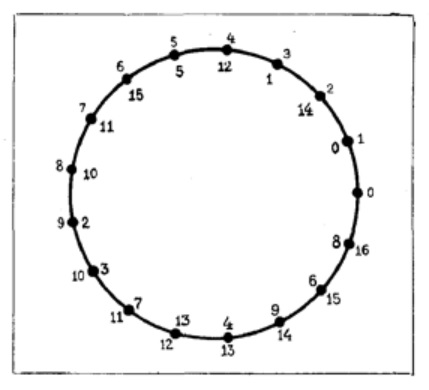
\includegraphics[scale=.8]{lab7.jpg}
\textbf{Рис. 7. Старые номера корней даны черным цветом, новые - красным.}
\vspace{90pt}

 16; затем $3^16$ дает остаток 1 и далее остатки повторяются (докажите!)
 
 Закономерность, подмеченная Гауссом, является частным случем следующей теоремы: 
\so{для всякого простого $p$ существует такое число $l$, называемое первообразным корнем, что среди остатков от деления $l^k$ на $p$ встерчаются все числа $1, 2, \ldots, p-1$}. Этот факт впервые отметил Эйлер (1707-1783), но смог доказать лишь Лежандр (1752-1833); другое доказательство получил Гаусс, но, вероятно, в 1796 году он еще не обладал теоремой, а обраружил приведенный факт эмпиричиски, проводя вычисления для конкретных чисел. Это очень важное обстоятельство, не учитывая которого, трудно правильно понять природу ранних работ Гаусса. Присвоим корню $\epsilon_k, k = 3^k$, новый номер, а именно $l$, который мы
\end{minipage}
\vspace{10pt}
\par\textbf{Таблица}
\vspace{10pt}

\begin{tabular}{ | l | l | l | l |l | l |l| l | l | l | l |l | l |l |l |l|l|}
\hline
0& 1 & 2 & 3 & 4& 5 & 6 & 7 & 8& 9 & 10 & 11 & 12& 13 & 14 & 15 & 16 \\ \hline
1 & 3 & 9 & 10 & 13 & 5& 15 & 11 & 16 & 14& 8 & 7 & 4 & 12 & 2& 6 & 1 \\
\hline
\end{tabular}
\vspace{10pt}
\par\textbf{6}

\vspace{50pt}

\par Используя неравенство $x y \le \frac{1}{2}(x^2 + y^2)$, напишем следующую цепочку неравенств: $\frac{\sum\limits_{i = 1}^n a_i b_i}{AB} = \sum\limits_{i = 1}^n \left(\frac{a_i}{A} \cdot \frac{b_i}{B}\right) \le$ 
$$
\le \sum\limits_{i = 1}^n \frac{1}{2}\left[ \left( \frac{a_i}{A}\right)^2 + \left( \frac{b_i}{B}\right)^2\right] = \frac{1}{2} \left( \frac{1}{A^2}\sum\limits_{i = 1}^n a_i^2 + \frac{1}{B^2} \sum\limits_{i = 1}^n b_i^2\right) = 1
$$
Отсюда следует неравенство $(*)$. Как известно, равенство в нем достигается при
$$
\frac{a_1}{A} = \frac{b_1}{B}, \frac{a_2}{A} = \frac{b_2}{B}, \ldots, \frac{a_n}{A} = \frac{b_n}{B}
$$
то есть при
$$
\frac{a_1}{b_1} = \frac{a_2}{b_2} = \ldots = \frac{a_n}{b_n}. 
$$
Покажем теперь, как применяется неравенство $(*)$.
